\documentclass[a4paper,titlepage,onecolumn]{report}
% title of the dissertation
\def\distitle{Coupled Systems in Single Molecule Biosensing}
\usepackage{todonotes}
\usepackage{mathtools}
\usepackage{t1enc}
\usepackage[T1]{fontenc}
\usepackage{ulem}
\usepackage{import}
\usepackage{amsmath}
\usepackage{amssymb}
\usepackage{paralist}
\usepackage{booktabs}
\usepackage[version=3]{mhchem}
\usepackage{wrapfig}
\usepackage{pifont}
\usepackage{mathrsfs}
\usepackage{tikz}
\usepackage{xcolor}
\usepackage{color}
\usepackage{enumitem}
\usepackage{datetime}
\usepackage{fullpage}
\usepackage{hyperref}
\usepackage[parfill]{parskip}


\hypersetup{
 colorlinks=true,
 citecolor=black,
 linkcolor=black,
 pdftitle={\distitle}
}

% New definition of square root:
% it renames \sqrt as \oldsqrt
% This definition puts a little vertical guy at the end so it's more
% obvious where the square root actually ends.
\let\oldsqrt\sqrt
% it defines the new \sqrt in terms of the old one
\def\sqrt{\mathpalette\DHLhksqrt}
\def\DHLhksqrt#1#2{%
\setbox0=\hbox{$#1\oldsqrt{#2\,}$}\dimen0=\ht0
\advance\dimen0-0.2\ht0
\setbox2=\hbox{\vrule height\ht0 depth -\dimen0}%
{\box0\lower0.4pt\box2}}

% integrals with infinity bounds
\newcommand{\intinfty}{\int_{-\infty}^{\infty}}

% consistent formatting of object labels
\newcommand{\Figure}[1]{Figure \ref{#1}}
\newcommand{\Equation}[1]{Equation \ref{#1}}
\newcommand{\Table}[1]{Table \ref{#1}}
\newcommand{\Section}[1]{Section \ref{#1}}
\newcommand{\Chapter}[1]{Chapter \ref{#1}}
\newcommand{\Part}[1]{Part \ref{#1}}
\newcommand{\Appendix}[1]{Appendix \ref{#1}}

% I want all of the document numbering to always show the full path, fuck
% with this later
%\renewcommand\thesection{\Roman{part}.\Alph{chapter}.\arabic{section}}
%\renewcommand\thesubsection{\arabic{section}.\arabic{subsection}}
%\renewcommand\thesubsubsection{\arabic{subsection}.\arabic{subsubsection}}

%\renewcommand\thefigure{S\arabic{figure}}
%\renewcommand\thesection{\Roman{part}.\arabic{chapter}.\arabic{section}}
%\renewcommand\thetable{S\arabic{table}}

% names have a particular formatting
\newcommand{\name}[1]{\textsc{#1}}

% missing mathematical operators
\DeclareMathOperator{\sinc}{sinc}
\DeclareMathOperator{\sech}{sech}
\DeclareMathOperator{\sgn}{sgn}
\DeclareMathOperator{\erf}{erf}
\DeclareMathOperator{\inverf}{inverf}
\DeclareMathOperator{\arcsinh}{arcsinh}
\DeclareMathOperator{\arccosh}{arccosh}
\DeclareMathOperator{\arctanh}{arctanh}
%\DeclareMathOperator{\Re}{Re}
%\DeclareMathOperator{\Im}{Im}

% use roman type for natural base e and sqrt(-1)
\newcommand{\me}{{\mathrm{e}}}
\newcommand{\mi}{{\mathrm{i}}}

% roman type for the derivative, plus a space
\newcommand{\md}{\,\mathrm{d}}

% fourier transform and the reverse
\newcommand{\ff}[1]{{\mathscr{F}^{+}\bigl(#1\bigr)}}
\newcommand{\fr}[1]{{\mathscr{F}^{-}\bigl(#1\bigr)}}

% hilbert transform and the reverse
\newcommand{\hf}[1]{{\mathscr{H}^{+}\bigl(#1\bigr)}}
\newcommand{\hr}[1]{{\mathscr{H}^{-}\bigl(#1\bigr)}}

% QCM related frequency and bandwidth shifts
\newcommand{\df}{\Delta\!f}
\newcommand{\dg}{\Delta\Gamma}
\newcommand{\xil}{\xi_\mathrm{L}}
\newcommand{\kl}{k_\mathrm{L}}
\newcommand{\ml}{m_\mathrm{L}}
\newcommand{\kq}{k_\mathrm{q}}
\newcommand{\mq}{m_\mathrm{q}}
\newcommand{\omegaq}{\omega_\mathrm{q}}

% custom lengths for figures

% width for side by side figures
\newlength{\twoupwidth}
\setlength{\twoupwidth}{7.5cm}

% width and height for default single figure
\newlength{\oneupwidth}
\setlength{\oneupwidth}{0.90\textwidth}
\newlength{\oneupheight}
\setlength{\oneupheight}{0.55623059\textwidth}

\usepackage{pgfplots}
\pgfplotsset{compat=newest}
\usepgfplotslibrary{units}
\usetikzlibrary{pgfplots.units}
\usetikzlibrary{calc}

\usepgfplotslibrary{units}
\usetikzlibrary{pgfplots.units} 

\import{colors/}{colors}

% siunitx
\usepackage{siunitx}
\DeclareSIUnit\molar{\mole\per\cubic\deci\metre}
\DeclareSIUnit\Molar{\name{M}}

\sisetup{ 
% load-configurations=abbreviations
% round-mode = places,
}%

\pdfpageattr {/Group << /S /Transparency /I true /CS /DeviceRGB>>} 

\begin{document}

%%%%% TITLE PAGE %%%%%
\begin{titlepage}
\begin{center}
\hfill\\[4cm]
{ \Huge {\bfseries {\distitle}} \par}
\vspace{3.0cm}
\begin{tabular}{lr}

\includegraphics[height=2cm,keepaspectratio]{logo/Logo_MPL_englisch_kompakt_cmyk_110915}
\hspace{1.0cm}
%

\includegraphics[height=2cm,keepaspectratio]{logo/Logo_IMPRS_4c_042012}
\end{tabular}
\vspace{3cm}
\\
{\huge Aaron Webster}\\
\vspace{1cm}
{\large A DISSERTATION}\\
\vspace{0.5cm}
Presented to the Max Planck Institute for the Science of Light\\
and the University of Erlangen-N\"urnberg\\
in partial fulfillment of the requirements\\
for the degree of\\
Doctor of Philosophy\\
\vspace{0.5cm}
\today
\end{center}
\end{titlepage}

%%%%% DECLARATION OF ORIGINALITY %%%%%
\chapter*{Declaration of Originality}
I affirm that the work presented in this dissertation is, to the best of my
knowledge, original and my own, except as acknowledged in the
text. \\
\hfill\\[1cm]
Signed\hspace{0.25cm}\makebox[5cm]{\hrulefill}\hspace{0.25cm}(Aaron Webster)
\hfill\\[1cm]
Date\hspace{0.51cm}\makebox[5cm]{\hrulefill}\hspace{0.25cm}
\vspace{2cm}

%%%%% ADVISOR, CO-ADVISOR %%%%%
\section*{Evaluation Committee}
\subsection*{First Advisor}
Dr. Rer. Nat. Frank Vollmer\\
Laboratory of Biophotonics and Biosensing\\
Max Planck Institute for the Science of Light\\
G\"unther-Scharowsky-Str.1 / Bau 24\\
91058 Erlangen
\subsection*{Second Advisor}
Prof. Dr. Ulf Peschel\\
Institute of Optics, Information and Photonics\\
University Erlangen-N\"urnberg\\
G\"unther-Scharowsky-Str.1 / Bau 24\\
91058 Erlangen

\newpage
%%%% ACKNOWLEDGEMENTS %%%%
\chapter*{Acknowledgements}
I would like to extend my sincerest gratitude to the following individuals
who contributed to this work: \name{Jiapeng~Huang}, for his enthusiasm
and hard work in carrying out many tedious but necessary experiments,
\name{Yuqiang~Wu} for establishing the DNA origami and related protocols,
\name{Matthew~Foreman} for carrying out insightful theoretical modeling
regarding SPP multiple scattering, \name{Frank~Vollmer} for his optimism
in seeing this work to a successful completion, \name{Stephen~Gregory}
and \name{R\@.P.\@~Schumann} whose pioneering experiments are the basis
for my own, and \name{Yuki~Sato} for his patience and progressive
scientific ideas regarding his centrifugal force quartz crystal
microbalance.  Most significantly, I would like to recognize
\name{Norbert~Lindlein}, without whom this dissertation would not exist.

%%%%% TABLE OF CONTENTS &&&&&
\pagenumbering{roman}
\tableofcontents

%%%%% ABSTRACT %%%%%
\begin{abstract}
 \todo{Abstract is written last.}
\end{abstract}
% the first part is in roman numbering, switch now to arabic
\pagenumbering{arabic}

\chapter*{Foreword}
The field of biosensing has this theme: very simple setups were though not
possible, but then were made relevant 

\todo{Summarize and give a quick overview of the different parts and what
they are good for.}

\part{Interference and Scattering in Surface Plasmon Resonance}
\label{part:plasmon}
\chapter{Preface}
\section{Synopsis}
This part is all about what happens when surface plasmons are
scattered in a prism coupled setup.  The easiest way of understanding this
is though the experimental setup, shown below in \Figure{fig:kretschmanngeo}.  
\begin{figure}[hb]
\centering
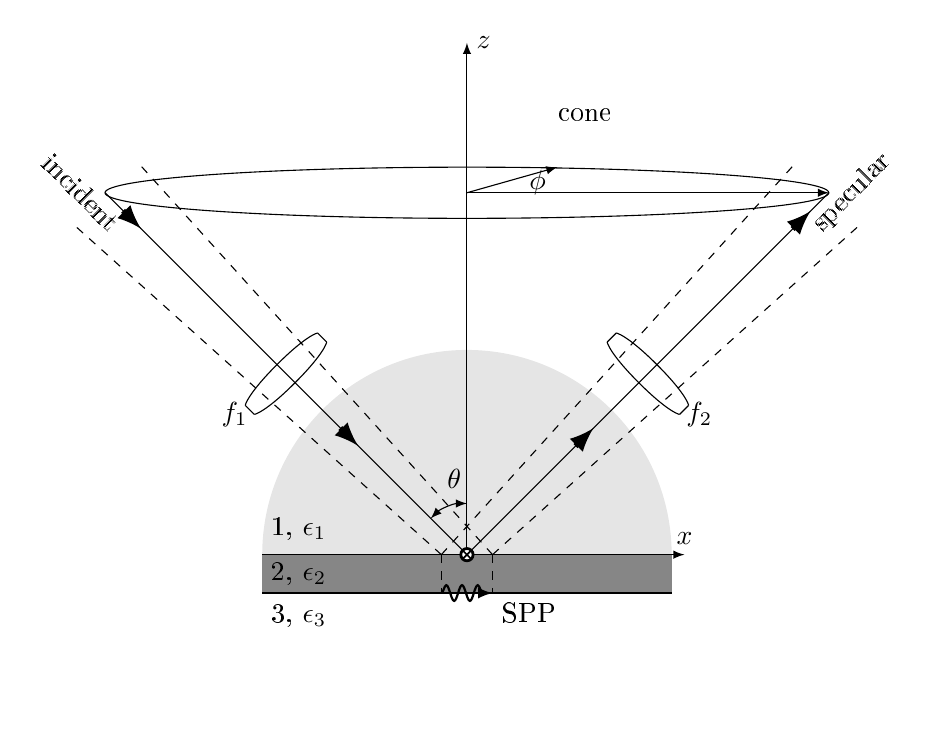
\begin{tikzpicture}[
    scale=0.65,
    >=latex,
    media/.style={font={}},
    wave/.style={
        decorate,decoration={snake,post length=1.0mm,amplitude=1mm,
        segment length=2.0mm},thick},
    interface/.style={
        % The border decoration is a path replacing decorator.
        % For the interface style we want to draw the original path.
        % The postaction option is therefore used to ensure that the
        % border decoration is drawn *after* the original path.
        postaction={draw,decorate,decoration={border,angle=-45,
                    amplitude=0.3cm,segment length=2mm}}},
    ]

    \def\thetasp{45}
    \def\spread{10}
    \def\wx{1}
    \def\conedist{10}

    % glass
    \fill[gray!20] (4,0) arc (0:180:4);

    % air
    \fill[gray!0] (-4,-3) rectangle (4,0);

    % metal
    \fill[gray!95] (-4,-0.75) rectangle (4,0);

    % Interface
    \draw[black,line width=.5pt](-4,0)--(4,0);
    \draw[black,line width=.5pt](-4,-0.75)--(4,-0.75);

    % Vertical dashed line
    %\draw[dashed,gray](0,-3)--(0,3);
    % Coordinates system
    \draw[<->] (4.25,0) node[above]{$x$}-|(0,10) node[right]{$z$};
    \draw[->] (0,{cos(\thetasp)*\conedist}) -- ({sin(\thetasp)*\conedist}, {cos(\thetasp)*\conedist});
    \draw[->] (0,{cos(\thetasp)*\conedist}) --
    ({0.25*cos(\thetasp)*\conedist}, {0.5+sin(\thetasp)*\conedist})
    node[shift={(-0.25,-0.20)}] {$\phi$} ;

    \node[shift={(1.5,{sin(\thetasp)*\conedist-1.5})}] {cone};

    % cone
    \draw (0,{cos(\thetasp)*\conedist}) ellipse ({sin(\thetasp)*\conedist} and 0.5);

    % Incidence
    %\draw[->,wave]
    %     (135:3.2cm)--(135:2.5cm)node[right]{$E_0$};
    \draw[dashed](0:{\wx*-0.5})--({90+\thetasp+\spread*0.5}:10);
    \draw[](0:0)--({90+\thetasp}:10) node[rotate={270+\thetasp}, shift={({0.30*cos(270-\thetasp)},{0.30*sin(270-\thetasp})}] {incident};
    \draw[<->] (0,1) arc (90:{90+\thetasp}:1) node[shift={(0.3,0.5)}] {$\theta$};
    \draw[->,line width=2pt]({90+\thetasp}:9.5)--({90+\thetasp}:9.0);
    \draw[->,line width=2pt]({90+\thetasp}:3.5)--({90+\thetasp}:3.0);
    \draw[dashed](0:{\wx*0.5})--({90+\thetasp-\spread*0.5}:10);
    %\draw[->](0,0.75)arc(90:135:.75cm);

    % Reflection
    %\draw[->,wave]
    %     (45:2.5cm)--(45:3.2cm)node[right]{$E_r$};
    \draw[dashed](0:{\wx*-0.5})--({90-\thetasp+\spread*0.5}:10);
    \draw[](0:0)--({90-\thetasp}:10) node[rotate={90-\thetasp},
    shift={({0.30*cos(270+\thetasp)},{0.30*sin(270+\thetasp})}] {specular};
    \draw[<-,line width=2pt]({90-\thetasp}:9.5)--({90-\thetasp}:9.0);
    \draw[<-,line width=2pt]({90-\thetasp}:3.5)--({90-\thetasp}:3.0);
    \draw[dashed](0:{\wx*0.5})--({90-\thetasp-\spread*0.5}:10);
    \draw[dashed]({\wx*0.5},0)--({\wx*0.5},-0.75);
    \draw[dashed]({-\wx*0.5},0)--({-\wx*0.5},-0.75);
    \draw[->,wave,color=black]
     ({-\wx*0.5},-0.75)--({\wx*0.5},-0.75) node[right,shift={(0,-0.25)}]{SPP};


    % first lens
    \def\lenswidth{2}
    \def\lensheight{0.25}
    \def\lensbow{0.125}
    \def\lensshift{({-5*sin(\thetasp)},{5*cos(\thetasp)})}
    \def\lensrotate{\thetasp}
    \draw[shift={\lensshift}, rotate={\lensrotate}]({-\lenswidth/2},{-\lensheight/2})--({-\lenswidth/2},{\lensheight/2});
    \draw[shift={\lensshift}, rotate={\lensrotate}]({\lenswidth/2},{-\lensheight/2})--({\lenswidth/2},{\lensheight/2});
 
    \draw[shift={\lensshift}, rotate={\lensrotate}] plot [smooth, tension=1.5] coordinates {
    ({\lenswidth/2},{-\lensheight/2})
    (0,{-\lensheight/2-\lensbow})
    ({-\lenswidth/2},{-\lensheight/2})
    } node[shift={(-0.25,0)}] {$f_1$};

    \draw[shift={\lensshift},rotate={\lensrotate}] plot [smooth, tension=1.5] coordinates {
    ({-\lenswidth/2},{\lensheight/2})
    (0,{\lensheight/2+\lensbow})
    ({\lenswidth/2},{\lensheight/2}) };
 
    % second lens
    \def\lensshift{({5*sin(\thetasp)},{5*cos(\thetasp)})}
    \def\lensrotate{-\thetasp}
    \draw[shift={\lensshift}, rotate={\lensrotate}]({-\lenswidth/2},{-\lensheight/2})--({-\lenswidth/2},{\lensheight/2});
    \draw[shift={\lensshift}, rotate={\lensrotate}]({\lenswidth/2},{-\lensheight/2})--({\lenswidth/2},{\lensheight/2});
 
    \draw[shift={\lensshift}, rotate={\lensrotate}] plot [smooth, tension=1.5] coordinates {
    ({-\lenswidth/2},{-\lensheight/2})
    (0,{-\lensheight/2-\lensbow})
    ({\lenswidth/2},{-\lensheight/2})
    } node[shift={(0.25,0)}] {$f_2$};

    \draw[shift={\lensshift},rotate={\lensrotate}] plot [smooth, tension=1.5] coordinates {
    ({-\lenswidth/2},{\lensheight/2})
    (0,{\lensheight/2+\lensbow})
    ({\lenswidth/2},{\lensheight/2}) };


   % Media names
    \path[media] (-4,.5)  node[anchor=west] {1, $\epsilon_1$}
                 (-4,-.375) node[anchor=west] {2, $\epsilon_2$}
                 (-4,-1.2) node[anchor=west] {3, $\epsilon_3$};

    % $x$ axis
    \filldraw[fill=white,line width=1pt](0,0)circle(.12cm);
    \draw[line width=.6pt] (0,0)
                          +(-135:.12cm) -- +(45:.12cm)
                          +(-45:.12cm) -- +(135:.12cm);
    % To-paths are really useful for drawing curved lines. The above
    % to path is equal to:
    %
    % \draw[-latex,thick](3.2,0.5)node[right]{$\mathsf{S_{1,2}}$}
    %      ..controls +(180:.2cm) and +(up:0.25cm) .. (3,0);
    % Internally the to path is translated to a similar bezier curve,
    % but the to path syntax hides the complexity from the user.

    % SPP
    %\draw[->,wave,color=black]
    %     (-2,-1.75)--(2,-1.75) node[right]{SPP};

\end{tikzpicture}

\vspace{-1cm}
\caption{
Experimental setup.
} 
\label{fig:kretschmanngeo} 
\end{figure}
Light is incident from the left and focussed by lens $f_1$ on to the
hypotenuse of a hemispherical prism coated with a thin layer of silver.
$f_2$ acts to image light exiting the system, if desired.

The evanescent wave present on the $\epsilon_1$-$\epsilon_2$ boundary with
a wavenumber $k_x = k_0\sqrt{\epsilon_1}\sin \theta$ has an angle such that
it excites surface plasmon polaritions (SPPs).  SPPs are oscillations of
free charge strongly coupled to the photons of the incident beam.  The
majority of light is directed into the specular direction.  Here,
re-radiated SPPs at $\theta_\mathrm{sp}$ are antiphase with the excitation
beam.  The result is interference: a dark band or notch in the reflected
field.  SPPs will propagate on the $\epsilon_2$-$\epsilon_3$ layer until
they either decay as heat or scatter into the far field.  During this
propagation it is possible that surface roughness will elastically modify
its $k$-vector in the $k_x$-$k_y$ plane.  When this happens, scattered SPPs
will re-radiate into a thin annular cone at (nearly) the same angle as the
dark band in the specular direction.

The conically scattered light is of prime importance in this work, because
within this light is found a wealth of information directly related to the
SPP scattering.  In particular, the cone contains speckle: a seemingly
random interference pattern resulting from many components with different
phase relationships.

\section{What is New Here}
In many large dissertations it is sometimes difficult to discern what is
actually new from rehashings of work others have done.  Here I intended to
clarify this situation.  To this accord, the following is a list of
explicitly new results which I present:

\begin{description}
\item[{Interference of Scattered SPPs}]
For SPPs excited in the Kretschmann configuration with a focussed beam
whose propagation distance is larger than focal spot, a one-sided
interference pattern, or ``wiggles'', is observed in the specular direction.  This was
thought to be an interference effect between the specularly reflected beam
and a re-radiated plasmon component, but we have discovered that that this is
simply a consequence of causality.
\item[{Bulk Refractive Index Sensitivity}] 
Using Fourier analysis, we have studied the sensitivity of SPR in an intensity
interrogation configuration as a function of propagation distance.  This
provides a useful measure of the sensitivity of the one-sided interference
pattern found in the specular and conically directed beams.
\item[{Refractive Index Sensing With Conical Speckle}]
If the surface is rough, the conically directed light contains speckle.  We
have analyzed the speckle patterns as a function of changes in bulk
refractive index.
\item[{SPP Nanoparticle Scattering}]
Using the speckle in the cone, we observe the changes in intensity and
correlation functions associated with the addition or motion of a single
nanoparticle.
\todo{After writing, update the list with all the new stuff.}
\end{description}

\section{Organization}
\todo{%
How the thesis is organized, what goes where and in what chapter
-- probably should do this part last.
}

\chapter{Foundations}
\section{Historical Perspective}
The theoretical groundwork for the existence of surface plasmon polaritons
(SPPs) was first introduced by \name{Richie} in his seminal 1957 paper
\textit{Plasma Losses by Fast Electrons in Thin Films}
\cite{ritchie1957plasma}.  Like any scientific work, Richie's was
incremental and has its roots in earlier theoretical proposals by
\name{Pines} and
\name{Bohm}~\cite{bohm1951collective}~\cite{pines1952collective}.
Ultimately this research functioned to explain the phenomena of sharp and
spectrally narrow energy losses observed in diffraction gratings by
\name{Wood} in 1902, known as ``Wood's anomaly''.

Optical excitation of surface plasmons was made accessible through
pioneering work in the late 1960's by
\name{Kretschmann}~\cite{kretschmann1968},
\name{Raether}~\cite{raether1965springer} and
\name{Otto}~\cite{otto1968excitation}.  These experiments used the
principle of attenuated total reflection (ATR) to excite surface plasmons
evanescently, using a prism to match their resonance condition.  A great
deal of understanding on the topic of surface plasmons took place in the
subsequent decade, including an improved theoretical understanding based on
Fresnel relations \cite{chen1976excitation} and descriptions of of
conically scattered light in the presence of surface
roughness~\cite{simon1976directional}.  A concise overview of this research
can be found in~\cite{raether1997surface}.

The introduction of SPR as a biosensing platform began in the early 1980's
with work by \name{Liedberg}, \name{Nylander} and
\name{Lundstrom}~\cite{liedberg1983surface} who described the
extraordinary sensitivity of the surface plasmon resonance condition to
perturbations in the refractive index of the medium on one side of the
metal film.  The subsequent commercialization of SPR biosensors has largely
been influenced by these authors and Pharmacia Biosensor AB (now
Biacore)~\cite{liedberg1995biosensing}.

The commercial success of biosensors based on surface plasmon resonance
brought about a knowledge gap between the biosensing community and their
more theoretical predecessors from whom the field owes its genesis; the
scope of SPR biosensing experiments is disproportionately narrower than the
breadth of phenomena discovered since Richie.  As an example particular to
this dissertation, in 2005 and 2007, two
papers~\cite{andaloro2005optical}~\cite{simon2007observation} based on
theoretical work by \name{Chuang}~\cite{chuang1986lateral} and
\name{Chen} \cite{chen1976excitation} reported a curious interference
pattern occurring in the specularly reflected light for certain (among
them, Kretschmann-Raether type) systems illuminated with focused Gaussian
beams.  This was also independently reported a year later in
\cite{schumann2008near}.  Interestingly, observation of this interference
required nothing more than the addition of a lens pair to a fairly
ubiquitous optical setup, but it somehow escaped attention during earlier
research.  

Many of the topics here are inspired by work done at the University of
Oregon in the labratory of \name{Stephen Gregory}, summarized in
a 2009 thesis \textit{Surface Plasmon Random Scattering and Related
Phenomena} \cite{schumann2009surface} by \name{R\@.P.\@~Schumann}.
Here is described experiments performed on thin metal films in a
Kretschmann-Raether configuration with the addition of a scanning
apertureless near-field probe.  This probe (a sharp tungsten tip) is able
to elastically scatter SPPs in a way analogous to surface roughness, but in
this case its location and interaction can be precisely controlled.
Lacking this apparatus, we can do similiar experiments using biological
affinities and gold nanoparticles.
\todo{Improve this last sentence.}

\section{Surface Plasmon Polaritons}
A photon is a quantized oscillation of an electromagnetic field.  When this
field is in proximity to an interface such as the surface of a metal,
oscillations of free charge can be induced.  If the field is evanescent in
both directions orthogonal to the surface, the oscillations become
localized and are known as surface plasmons (SPs).  Furthermore, if
conditions exist such that the in-plane momentum and phase of the incident
photon and the surface plasmon match, the coupling produces a hybrid
excitation known as surface plasmon polariton (SPP).  An SPP is trapped on
this interface and propagates until it decays; either re-radiating as a
photon or being absorbed into the metal as heat.

SPPs, like photons, are quantum mechanical objects.  Because this system is
largely momentum-conserving, elastically scattered plasmons will preserve
all the information of their parent field.  There are many well written
treatments which derive SPPs from many different types of first principles.
Since this has already been done, I will simply sumarize the relevant
mathematics.

\subsection{Wave Equation}
Most of the relevant behavior of SPP propagation can be derived from the
electromagnetic wave equation derived from Maxwell's equations.
\begin{align}
\left(\nabla^2-\mu\epsilon\frac{\partial^2}{\partial t^2}\right)\mathbf{E}&=0
\label{eqn:ewe}
\end{align}
This is the electromagnetic wave equation in terms of the electric field.
Choosing to solve this equation by separation of variables the following
plane wave solutions can be obtained
\begin{align}
 \mathbf{E} ( \mathbf{r}, t ) &= \mathbf{E}_0\, \me^{\mi (\mathbf{k} \cdot \mathbf{r} - \omega t )}
\label{eqn:planewaves}
\end{align}
where $k=\omega/c=\omega\sqrt{\epsilon\mu}$.  In this notation,
$\mathbf{k}$ is the material specific vectorial wavenumber, $\mathbf{r}$ is the
spatial position, $\omega$ is angular frequency, and $t$ is
the dimension of time.
The initial value is chosen with the vectorial constant $\mathbf{E}_0$.
The magnetic field follows the same form
\begin{align}
 \mathbf{H} ( \mathbf{r}, t ) &= \mathbf{H}_0\, \me^{\mi (\mathbf{k}
 \cdot \mathbf{r} - \omega t )}
\end{align} 
but it is orthogonal $\mathbf{E}$ by
\begin{align}
\mathbf{E} \times \mathbf{H} = 0
\end{align}
and the two are mutually orthogonal with the direction of propagation
$\mathbf{k}$.

\subsection{Dispersion Relation}
With plane wave solutions in hand, boundary conditions consistent with a
dielectric-metal interface can be imposed.
At a planar interface, it is convenient to restrict the problem to two
dimensions; in this case the $x$-$z$ plane as shown schematically in
\Figure{fig:kretschmanngeosimplified}.  Since $\mathbf{k}=(k_x,0,k_z)$,
$\mathbf{r}\cdot\mathbf{k}=k_x x + k_z z$ and $\mathbf{E}_0 = (E_x, 0,
E_z)$, the electric field can be written 
\begin{align}
\mathbf{E} ( \mathbf{r}, t ) &= \mathbf{E}_0\, \me^{\mi (\mathbf{k}
\cdot \mathbf{r} - \omega t )}\\
\mathbf{E}(x,z,t)&=\begin{pmatrix}
E_x\\ 0\\ E_z
\end{pmatrix}
\, \me^{\mi(k_{x,i}x+k_{z,i}z-\omega t)}
\label{eqn:planewavexz}
\end{align}
The magnetic field propagates in the same direction with the
same $\mathbf{k}$-vector components, but the direction
$\mathbf{H}$ must be orthogonal to $\mathbf{E}$ by
\Equation{eqn:faradayslaw}
\begin{align}
\mathbf{H} ( \mathbf{r}, t ) &= \mathbf{H}_0\, \me^{\mi (\mathbf{k}
\cdot \mathbf{r} - \omega t )}\\
\mathbf{H}(x,z,t)&=\begin{pmatrix}
0\\ H_y\\ 0
\end{pmatrix}
\, \me^{\mi(k_{x,i}x+k_{z,i}z-\omega t)}
\end{align}
At the interface there are two values for the (complex) permittivity,
$\epsilon_1$ in the dielectric and $\epsilon_2$ in the metal.  Consequently
there are two sets of plane wave solutions
\begin{align}
\left.\begin{aligned}
\mathbf{H}_1(x,z,t) &=
\begin{pmatrix}
0\\
H_{y,1}\\
0
\end{pmatrix} \me^{\mi(k_{x,1}x+k_{z,1}z-\omega t)}\\
\mathbf{E}_1(x,z,t) &=
\begin{pmatrix}
E_{x,1}\\
0\\
E_{z,1}\\
\end{pmatrix} \me^{\mi(k_{x,1}x+k_{z,1}z-\omega t)}
\end{aligned}
\right\}& \quad \text{dielectric}, \epsilon_1\label{eqn:planewavedielectric}\\
\left.\begin{aligned}
\mathbf{H}_2(x,z,t) &=
\begin{pmatrix}
0\\
H_{y,2}\\
0
\end{pmatrix}
\me^{\mi(k_{x,2}x+k_{z,2}z-\omega t)}\\
\mathbf{E}_2(x,z,t) &=
\begin{pmatrix}
E_{x,2}\\
0\\
E_{z,2}\\
\end{pmatrix}
\me^{\mi(k_{x,2}x+k_{z,2}z-\omega t)}
\end{aligned} 
\right\}&\quad \text{metal}, \epsilon_2
\label{eqn:planewavemetal}
\end{align}
where the subscript designates which material the wave equation refers to.
(e.g. $\mathbf{E}_1$ is the electric field in the dielectric, $\mathbf{H}_2$
the magnetic field in the metal, etc.)
Continuity of \Equation{eqn:planewavedielectric} and
\ref{eqn:planewavemetal} at this interface requires that
\begin{align}
E_{x,2}&=E_{x,1}\\
H_{y,2}&=H_{y,1}\\
\epsilon_2 E_{z,2}&=\epsilon_1 E_{z,1}
\end{align}
Applying Ampere's law (\Equation{eqn:ampereslaw}) to the field on the
each boundary gives
\begin{align}
\nabla \times \mathbf{H}_i &= \epsilon_i \frac{\partial \mathbf{E}_i}{\partial t}\\
\begin{pmatrix}
\frac{\partial H_{z,i}}{\partial y} - \frac{\partial H_{y,i}}{\partial z}\\
\frac{\partial H_{x,i}}{\partial y} - \frac{\partial H_{z,i}}{\partial z}\\
\frac{\partial H_{y,i}}{\partial y} - \frac{\partial H_{x,i}}{\partial z}
\end{pmatrix}
&= \begin{pmatrix}
-\mi k_{z,i} H_{y,i}\\
0\\
\mi k_{x,i} H_{y,i}
\end{pmatrix}
\\
&= \begin{pmatrix}
-\mi \omega \epsilon_i E_{x,i}\\
0\\
-\mi \omega \epsilon_i E_{z,i}
\end{pmatrix}
\label{eqn:vectordisp}
\end{align}
where $\mathbf{E}_i$, $\mathbf{H}_i$, $i=1,2$ represent the field in either the
dielectric or the metal.  The vector components of
\Equation{eqn:vectordisp} are therefore related 
\begin{align}
-\mi k_{z,i} H_{y,i} &= -\mi \omega \epsilon_i E_{x,i}\\
k_{z,1} H_{y,1} &= \omega \epsilon_1 E_{x,1}\\
k_{z,2} H_{y,2} &= \omega \epsilon_2 E_{x,2}
\label{eqn:spderivsteptwo}
\end{align}
Since the components of both $\mathbf{E}_i$ and $\mathbf{H}_i$ are
parallel to the interface, $E_{x,i}$ and $H_{y,i}$ are also
continuous. By substitution of $E_{x,i}$, \Equation{eqn:spderivsteptwo} becomes
\begin{align}
\frac{k_{z,1}}{\epsilon_1}H_{y,1}&=\frac{k_{z,2}}{\epsilon_2}H_{y,2}\\ 
\Aboxed{
\frac{k_{z,1}}{\epsilon_1}&=\frac{k_{z,2}}{\epsilon_2} 
}
\label{eqn:sprcondition}
\end{align}
This is the surface plasmon resonance condition.  In terms of
its vector components, the following holds in general for all electromagnetic
waves
\begin{align}
\mathbf{k}^2=\epsilon_i \left(\frac{\omega}{c}\right)^2=k_x^2 + k_{z,i}^2\\
\epsilon_i k_0^2=k_x^2 + k_{z,i}^2
\label{eqn:dispersion1}
\end{align}
Substitution of \Equation{eqn:sprcondition} with the relation 
$k_{x,1}=k_{x,2}$ into \Equation{eqn:dispersion1} allows 
$k_x$ and $k_{z,i}$ to be rewritten in the form of a dispersion relation
\begin{align}
k_x &= k_0\sqrt{\frac{\epsilon_1 \epsilon_2}{\epsilon_1+\epsilon_2}} 
= \frac{\omega}{c}\sqrt{\frac{\epsilon_1 \epsilon_2}{\epsilon_1+\epsilon_2}}\\
k_{z,i} &= k_0\frac{\epsilon_i}{\sqrt{\epsilon_1+\epsilon_2}}
= \frac{\omega}{c}\frac{\epsilon_i}{\sqrt{\epsilon_1+\epsilon_2}}
\end{align}

This relation, shown in \Figure{fig:dispersionrelation}, is useful because
it shows graphically the condition under which SPPs may exist: at the
intersection between the photon light line and corresponding SPP light line
for the medium in question.  Note that for a photon and a plasmon in both a
vacuum and a dielectric, this never happens; the photon assumes $\omega = c
k /\sqrt{\epsilon_i}$ for $i=1,2$, diverging to infinity while the SPP
asymptotically approaches $\omega_p/\sqrt{1+\epsilon_i}$ as $k_x\to\infty$.
However, if light is incident from a dielectric $\epsilon_1$ at an angle
$\theta$, the slope of $\omega(k_x)$ is modified to $c k \sin
\theta/\sqrt{\epsilon_1}$ and the dispersion relations can be matched.
This is the principle exploited by Kretschmann \cite{kretschmann1968} to
excite SPPs with prisms.

There are several regions of interest in \Figure{fig:dispersionrelation},
depending on the relative value of $\epsilon_1$ and $\epsilon_2$.  We first
assume that $\epsilon_1$ is a dielectric with $\epsilon_1\in\mathbb{R}$ and
$\epsilon_1 > 0$ (true for most if not all glass).  In this case, for
$\Re(\epsilon_2)>0$, both $k_x$ and $k_z$ are real.  These are known as
``radiative modes'' -- an SPP mode is supported normal to the interface but
it is not bound there.  For $-\epsilon_1<\Re(\epsilon_2)<0$, $k_z$ is real
and $k_x$ imaginary.  The SPP is not confined to the interface and decays
evanescently there; this is known as a ``quasi-bound mode''  However, for
$\Re(\epsilon_2)<-\epsilon_1$, $k_x$ is real and $k_z$ is imaginary.  This
indicates the SPP is localized at the interface in $z$ while having a
propagating solution in $x$, and is exactly the condition we wish to match.
\begin{figure}[ht]
\centering
\begin{tikzpicture}
\begin{axis}[
xlabel=$k_x$,
ylabel=$\omega$,
xmin=0,
xmax=0.6e8,
ymin=0.75e15,
ymax=6.5e15,
thick,
width=0.75\textwidth,
height=0.75\textwidth,
minor tick num=2,
legend pos = south east,
legend style = { cells = {anchor=west} },
clip=false,
]
\addplot[color=Dark27qual1] file {dispersion/kx_photon_glass.dat}
node [anchor=south west,yshift=-10pt]{$ck/\sqrt{\epsilon_1}$}; 
\addlegendentry{photon/dielectric}

\addplot[color=Dark27qual2] file {dispersion/kx_photon_glass_tilted.dat}
node [anchor=south west,yshift=-10pt]{$ck \sin \theta /\sqrt{\epsilon_1}$};
\addlegendentry{photon/dielectric angle}

\addplot[color=Dark27qual3] file {dispersion/kx_photon_vacuum.dat}
node [anchor=south west,yshift=-10pt]{$ck$}; 
\addlegendentry{photon/vacuum}

\addplot[color=Dark27qual4] file {dispersion/kx_sp_metal_glass_lower.dat};
\addlegendentry{SPP/dielectric}

\addplot[color=Dark27qual5] file {dispersion/kx_sp_metal_vacuum_lower.dat};
\addlegendentry{SPP/vacuum}

\addplot[color=Dark27qual1] file {dispersion/kx_sp_metal_glass_upper.dat};
\addplot[color=Dark27qual2] file {dispersion/kx_sp_metal_vacuum_upper.dat};

\addplot[color=Dark27qual1,dashed] coordinates { (6e7,5.819396016587478e+15) (0,5.819396016587478e+15) }
node [anchor=east,xshift=-15pt]{$\omega_p$}; 

\addplot[color=Dark27qual2,dashed] coordinates { (6e7,5.461458222933e+15) (0,5.461458222933e+15) }
node [anchor=east,xshift=-15pt]{$\omega_p/\sqrt{2}$}; 

\addplot[color=Dark27qual3,dashed] coordinates { (6e7,4959276840790959) (0,4959276840790959) }
node [anchor=east,xshift=-15pt]{$\omega_p/\sqrt{1+\epsilon_2}$}; 


\draw [decorate,decoration={brace,amplitude=8pt}] (axis cs:6e7,6.5e+15)--(axis cs:6e7,5.819396016587478e+15)
node [midway,anchor=west,xshift=10pt,align=left]{radiative modes\\ $k_x,k_z \in \mathbb{R}$};

\draw [decorate,decoration={brace,amplitude=8pt}] (axis cs:6e7,5.819396016587478e+15)--(axis cs:6e7,4959276840790959)
node [midway,anchor=west,xshift=10pt,align=left]{quasi-bound modes\\ $k_x \in \mathbb{I}$,  $k_z \in \mathbb{R}$};

\draw [decorate,decoration={brace,amplitude=8pt}] (axis cs:6e7,4959276840790959)--(axis cs:6e7,0.75e+15)
node [midway,anchor=west,xshift=10pt,align=left]{bound modes\\ $k_x \in \mathbb{R}$\\ $k_z \in \mathbb{I}$};

\end{axis}
\end{tikzpicture}
\caption{Dispersion relation for photons and plasmons.  Conditions under
which SPPs may occur at the intersection between the photon light line and
corresponding SPP light line for the medium in question.  Based on a
similar plot found in \cite{shsongspp}.}
\label{fig:dispersionrelation}
\end{figure}
\todo{Fix the colors here.}
%The dispersion diagram relates the time-variation of the wave (given by its
%frequency &omega) to the spatial variation of the wave (given by its
%wave-vector kx)
\subsection{Resonance Condition}
The resonance condition requires the dispersion relation for an
incident photon intersect the dispersion relation for SPPs, matching both
their in-plane momentum and phase.  This can be achieved by if the photon
is indecent through a dielectric at an $\theta_\text{sp}$, causing its phase
velocity $\omega/k_x$ to be reduced to  $\omega/k_x = c/(\sqrt{\epsilon_1}
\sin \theta)$.  One simple and popular prism coupled configuration (the one
which will be employed throughout this work) which is able to match these
conditions is known as the Kretschmann attenuated total reflection (ATR)
configuration, and is shown schematically in \Figure{fig:kretschmanngeo}.
Here a thin ($\sim \SI{50}{\nano\meter}$) metal film is deposited on to the
hypotenuse of a dielectric prism, and the totally internally reflected
light evanescently excites SPPs.  The SPP resonance condition for this
system is
\begin{align}
k_\text{sp}=k_0 \sqrt{\epsilon_1} \sin \theta_\text{sp} 
\end{align}
Note that practically this can only occur when both the width of the metal
layer $d$ is less than the evanescent decay in that direction
$\Im(1/k_{z,2})$ (causing the metal to be nearly transparent) and the
incident light satisfies the condition for total internal reflection.  This 
is approximately when
\begin{align}
\theta>\arcsin\left(\sqrt{\frac{\epsilon_1}{\epsilon_3}}\right)
\end{align} 
In practice the resonance angle $\theta_\text{sp}$ is most easily found by
numerically evaluating the Fresnel relations discussed in the following
section.

\subsection{Fresnel Relations}
Many features of surface plasmon resonance can be predicted using the
Fresnel relations and the transfer matrix method (TMM) for multilayer
stacks.
The Fresnel reflection coefficient $\tilde{r}$ is defined as the ratio of the
reflected beam $\tilde{E}_r$ to the incident beam
$\tilde{E}_i$
\begin{align}
\tilde{r} &= \frac{\tilde{E}_r}{\tilde{E}_i}
\end{align}
Here the presence of a tilde $\sim$ indicates a function in the (spatial)
frequency domain.  For multilayer systems, this is found through
the transfer matrix method where the $i$th matrix $M_i$ is
\begin{align}
M_i = \left(\begin{array}{cc}
\cos \sigma_i & \mi \sin \sigma_i / \gamma_i\\
\mi \gamma_i \sin \sigma_i & \cos \sigma_i
\end{array}\right)
\label{eqn:tmm}
\end{align}
and the system matrix $M_s = M_1 M_2 \ldots M_{n-1} M_n$.  In the above
representation
\begin{align}
\left.\begin{aligned}
\gamma_i &= \sqrt{\epsilon_i} k_{z,i}\\
\sigma_i &= k_{z,i} \sqrt{\epsilon_i} d_i
\end{aligned}
\right\}& \quad \text{for TE Polarization}\\
\left.\begin{aligned}
\gamma_i &= \sqrt{\epsilon_i}/k_{z,i}\\
\sigma_i &= k_{z,i} \sqrt{\epsilon_i} d_i
\end{aligned}
\right\}& \quad \text{for TM Polarization}
\end{align}
The elements of the resulting elements of $M_s$, $M_{i,j}$ are then
substituted into the formula
\begin{align}
\tilde{r}=
\frac{\gamma_1 M_{11}+\gamma_1 \gamma_3 M_{12} - M_{21} - \gamma_3 M_{22}}
{\gamma_1 M_{11}+\gamma_1 \gamma_3 M_{12} + M_{21} + \gamma_3 M_{22}}
\end{align}
With a bit of algebra, the Fresnel reflection for an arbitrary number of
layers in the case of TM polarization can be found to be
\begin{align}
\tilde{r}_{j,l,m \ldots n} = 
\frac{\tilde{r}_{j,l} + \tilde{r}_{l,m \ldots n} \me^{2 \mi k_{z,l} d_l}}
{1+\tilde{r}_{j,l} \tilde{r}_{l,m \ldots n} \me^{2 \mi k_{z,l} d_l}}
\label{eqn:bertnlayer}
\end{align}
where $d_l$ is the thickness of the $l$th metal layer and 
\begin{align}
\tilde{r}_{i,j}&=
\left.\left(\frac{k_{z,i}}{\epsilon_i}-\frac{k_{z,j}}{\epsilon_j}\right)
\middle/
\left(\frac{k_{z,i}}{\epsilon_i}+\frac{k_{z,j}}{\epsilon_j}\right)\right.\\
&=\frac{\epsilon_j k_{z,i}-\epsilon_i k_{z,j}}
{\epsilon_j k_{z,i}+\epsilon_i k_{z,j}}
\end{align}
is the two layer Fresnel relation.  \Equation{eqn:bertnlayer} may be
recursively applied for any number of layers.  There are computational
limits to this approach which make it unsuitable for large multilayer
stacks; in such a case methods based on \Equation{eqn:tmm} are more
appropriate.  For convience we state the three layer Fresnel reflectivity
$\tilde{r}_{123}$, based on the geometry of \Figure{fig:kretschmanngeo}
\begin{align}
\tilde{r}_{123}(k_x) &=
\frac{
  (\epsilon_2 k_{z,1}+\epsilon_1 k_{z,2})(\epsilon_3 k_{z,2}-\epsilon_2 k_{z,3})
+ (\epsilon_2 k_{z,1}-\epsilon_1 k_{z,2})(\epsilon_3 k_{z,2}+\epsilon_2 k_{z,3})\,
\me^{\mi 2 k_{z,2} d_2}
}
{
  (\epsilon_2 k_{z,1}+\epsilon_1 k_{z,2})(\epsilon_3 k_{z,2}+\epsilon_2 k_{z,3})
+ (\epsilon_2 k_{z,1}-\epsilon_1 k_{z,2})(\epsilon_3 k_{z,2}-\epsilon_2 k_{z,3})\,
\me^{\mi 2 k_{z,2} d_2}
}\\
&=
\frac{\tilde{r}_{12}+\tilde{r}_{23}\, \me^{\mi 2 k_{z,2} d_2}} {1+\tilde{r}_{12} \tilde{r}_{23} \me^{\mi 2 k_{z,2} d_2}}
\label{eqn:fresnel123}
\end{align}
Note that factor of two in the exponential: the SPP accumulates phase
through the metal film twice (once upon excitation, another upon decay).
In this equation, $k_{z,i}$ can be equivalently expressed either as a
function of incident angle $\theta$ or $k_x$
\begin{align}
k_{z,i} &= k_0 \sqrt{\epsilon_i - \epsilon_1 \sin \theta}\\
&= \sqrt{k_0^2\epsilon_i - k_x^2}
\end{align}\begin{flushleft}\begin{center}\end{center}\end{flushleft}
\subsection{Physical Properties}
The physical properties of SPP propagation are derived from $k_x$ and $k_z$.
Since the SPP is confined to the plane of the metal, the surface plasmon
wavelength $\lambda_\text{sp}$ is defined in terms of the real part of
$k_x$
\begin{align}
\lambda_\text{sp} &= \frac{\lambda_0}{2 \pi} k_x\\
& = \Re\left(\sqrt{
  \frac {\epsilon_1+\epsilon_2}
   {\epsilon_1 \epsilon_2 \lambda_0^2}
}\right)
\end{align}
when $k_x$ is imaginary, \Equation{eqn:planewavexz} is evanescent in
$x$ and the SPP decays with a characteristic $1/\me$ lifetime
$\Im(1/(2k_x)$.  Similarly, when $k_{z,i}$ is imaginary, the
$1/\me$ evanescent decay into either the metal or vacuum is given by
$\Im(1/k_{z,i})$.  A table of these properties for many different SPP
excitation configurations is found in \Appendix{ref:physicalproperties}.


\section{Experimental Setup}
\todo{Write here about how the experiment is done so there will be no
confusion later.}

\section{Long Range Surface Plasmon Polaritons}
The typical propagation distances for SPPs in the three layer Kretschmann configuration are on the order of $\SI{30}{\micro\meter}$ for Ag films and $\SI{6}{\micro\meter}$ for Au films.  The reason for this is the electric field extends into the metal and the real part of the metal's dielectric function damps the SPP oscillation, causing it to decay as heat.  However, if we are able to expel the SPP evanescent field from the metal region, the propagation distances can be extended orders of magnitude.  These are called \textit{long range surface plasmon polaritons} (LRSPPs), and in terms of our geometry can be excited in one of two ways.
\subsection{Symmetric Configuration}
Cytop coating crap
\subsection{Photonic Crystal Configuration}

\chapter{Interference}
Don't say this, but maybe say something like it
Surface plasmon resonance is in of itself an interference phenomena: the dark band in the specular direction is due to interference between
specularly reflected light and the re-radiated SPP which is likewise
antiphase at the SPR resonance angle.  There is, however, a more rich 
interference structure which can observed when using a focused beam whose spot size is smaller than the SPP propagation distance.  

\section{Interference in Surface Plasmon Resonance}
Perhaps the most 

\section{The Fourier Optics Perspective}
There are several perspectives of SPR phenomena which can be insightful in
explaining why exactly the spatial oscillations are one-sided.  The first
is an argument from causality.  Assume a complex function $\chi(\omega) =
\chi'(\omega) + \mi \chi''(\omega)$ whose real and imaginary parts are
related by Kramers-Kronig relations
\begin{align}
\chi(\omega)=\mi \hf{\chi(\omega)}
\end{align}
with 
\begin{align}
\chi'(\omega) &= \hf{\chi''(\omega)}\\
\chi''(\omega) &= -\hf{\chi'(\omega)}
\end{align}
where $\hf{\chi(\omega)}$ is the Hilbert transform of $\chi(\omega)$.
The Fourier transform of $\chi(\omega)$ is
\begin{align}
\chi(\omega) &= \chi'(\omega) + \mi \chi''(\omega)\\
\ff{\chi(\omega)} &= \ff{\chi'(\omega) + \mi \chi''(\omega)}\\
&= \ff{\chi'(\omega)} + \ff{\mi \chi''(\omega)}\\
&= \ff{\chi'(\omega)} + \ff{\mi \hf{\chi'(\omega)}} \\
&= \ff{\chi'(\omega)} + \sgn(\omega) \ff{\chi'(\omega)} \\
\end{align}
Or succinctly,
\begin{align}
\ff{\hf{\chi(\omega)}} = (-\mi \sgn(\omega)) \ff{\chi(\omega)}
\end{align}
In other words, the Fourier transform of any function which satisfies
Kramers-Kronig relations is ``one-sided'' as a necessary
condition of causality.  This seems to be true for the Fresnel
reflectivity as well as the complex permittivity.

The second perspective is couched in Fourier optics.  Here, because
SPR occurs at the focus of a Gaussian beam, it can be seen as a sort of
spatial filter which modifies the local $k$-vectors to produce
the resulting far field optical pattern.  If the SPR resonance condition is
sharp, the Fourier integral (\Equation{eqn:fourier123}) is truncated and
the discontinuity acts as a low pass filter for light.  The one-sided
oscillations are then essentially a manifestation of Gibb's phenomena.
This seems to be well supported, because if the SPR resonance is broadened,
say in the case of a BK7-Au-\ce{H2O} system, the interference is greatly
attenuated.
%
%Another possible interpretation is that the near and
%far field patterns in conically scattered light are qualatatively identical
%to the simple impulse-response of a forced, damped harmonic oscillator.
%This is of course equivalent to what the Lorentz-Drude model says about the
%material properties.  The far field conically scattered light likewise
%appears to be equivalent to the energy absorbed in the metal film which can
%be detected as heat.

\subsection{Specularly Directed Light}


\subsection{Spatial Evolution}
The Fresnel reflectivity predicts the far field angular distribution when
illuminated by light at a specific angle, consisting of a single
$k$-vector.  Now we will look at the evolution of light from this system
as it propagates to the far field when excited by an incident Gaussian beam
$g(x)$ containing a continuum of $k$-vectors.  We begin with treatment of
light in the specular direction.  In the context of Fourier
optics, the field on the surface in $k$-space is described by the Fourier
decomposed incident Gaussian beam $\tilde{g}(k_x)$ multiplied by the
Fresnel reflectivity
\begin{align}
\tilde{E}_\text{spec}(k_x)=\tilde{g}(k_x)\,\tilde{r}_\text{123}(k_x)
\end{align}
where
\begin{align}
\tilde{g}(k_x) = \intinfty g(x)\, \me^{\mi k_x x} \md x
\end{align}
and $g(x)$ represents a Gaussian beam in spatial dimensions.  We omit any 
specific definition for $g(x)$ because its exact form
is not important to our analysis.

The complete optical field in both $x$ and $z$ can be obtained by computing
the Fourier transform of $\tilde{E}_\text{spec}(k_x)$ multiplied 
by the free space transfer function $\me^{\mi k_{z,1} z}$
\begin{align}
E_\text{spec}(x,z) &= \intinfty \tilde{E}_\text{spec}\, \me^{\mi k_{z,1} z}\, \me^{\mi k_x x} \md k_x\\
 &= \intinfty \tilde{g}(k_x)\, \tilde{r}_{123}(k_x)\, \me^{\mi \sqrt{k_0^2 \epsilon_1 - k_x^2}z}\, \me^{\mi k_x x} \md k_x
\label{eqn:fourier123}
\end{align}
Likewise, conically scattered light may be found using the same treatment
\begin{align}
E_\text{cone}(x,z) = \intinfty \tilde{g}(k_x)\, \tilde{r}_{321}(k_x)\,\me^{\mi k_{z,1} z}\, \me^{\mi k_x x} \md k_x
\label{eqn:fourier321}
\end{align}
Though this integral seems to have no analytic solution, its evaluation is
nonetheless straightforward on a computer.
The evolution of scattered and specularly directed light based on
\Equation{eqn:fourier123} and \Equation{eqn:fourier321} is shown in
\Figure{fig:fresnelpropagate} as a function of distance from the 2-3
interface.  As can be seen, as the field propagates it diffracts,
displaying a one-sided oscillatory structure. 

\subsubsection{Evanescent Solutions}
In the context of diffraction integrals, the free space transfer function
$\exp(\mi k_{z,1} z)$ is often concerned with evanescent and propagating
terms, giving rise to the diffraction limit.  Here,
$k_{z,1}=\sqrt{k_0^2 \epsilon_1 - k_x^2}$ is imaginary for $k_0^2
\epsilon_1 < k_x^2$.  It is interesting to note that this never occurs.
Ignoring the condition for total internal reflection, 
$k_x = k_0 \sqrt{\epsilon_1} \sin \theta$ and we can set up an inequality
\begin{align}
k_0^2 \epsilon_1 &< k_x^2\\
k_0^2 \epsilon_1 &< \left(k_0 \sqrt{\epsilon_1} \sin \theta\right)^2\\
k_0^2 \epsilon_1 &< k_0^2 \epsilon_1 \sin^2 \theta\\
1 &< \sin^2 \theta
\end{align}
which is false, suggesting that if all light is collected, no information is
lost during propagation from the near to far field.


\chapter{Bulk Sensitivity}
The sensitivity of surface plasmon based biosensors to bulk refractive
index changes is of primary importance in extracting bio-relevant
properties. In a prism coupled setup, there are three main modulation
methods used to monitor changes in the SPR resonance.

\begin{description}
 \item [{Angular}] The prism is rotated and the signal reflectivity
  monitored
  as a function of angle. The prism may be scanned through a range of
  angles or the angular spectrum may be obtained simultaneously using
  a focussed beam and sensor array.
 \item [{Wavelength}] The prism is fixed in place and its reflectivity at
  a single angle is monitored as a function of wavelength.
 \item [{Intensity}] The intensity of the signal at a certain angular or
  spatial point is monitored as the experiment progresses.
\end{description}
All three of these interrogation methods are equivalent in terms of
their real-world resolution and detection limit. In this section we
will look at the sensitivity of intensity interrogation to different
(something about parameters)


\section{Three Layer Kretschmann, Far Field}
We will now derive the sensitivity of the three layer Kretschmann
configuration to bulk index changes. This case will be used as a test
case for further analysis of the propagation dependent sensitivity.

The bulk sensitivity in an intensity modulation setup is defined as
the ratio of the change of normalized signal intensity $\delta I=I_{n_{0}}-I_{n_{1}}$
to the change in bulk refractive index $\delta n=n_{0}-n_{1}$ for
two refractive indicies $n_{0}$ and $n_{1}$. We restrict ourselves
to small changes in the refractive index $n$, $\delta n/n_{0}\ll1$.
The intensity sensitivity is defined as
\begin{equation}
S_{\mathrm{I}}=\frac{\delta I}{\delta n}
\end{equation}
Without loss of generality, the sensor intensity $I$ may be a function
of any appropriate coordinate system (e.g. $I(x,y)$). In such a coordinate
system we always take $S_{\mathrm{I}}$ at the location of maximum
shift in that coordinate system.

In the Lorentzian approximation{[}{]} using Drude model coefficents
$\epsilon=\epsilon'+\mi\epsilon''$, the maximum sensitivity for bulk
index sensing is approximated as
\begin{equation}
(S_{\text{I}})_{\text{max}}=\frac{4\sqrt{3}}{9}\frac{\epsilon_{\mathrm{m}}'}{\epsilon_{\mathrm{m}}''n^{3}}
\end{equation}
Where $\epsilon_{\mathrm{m}}$ is the complex Drude-model permittivity
in the metal layer. At a operating wavelength of \SI{660}{\nano\meter},
for Au on N-BK7, $(S_{\mathrm{I}})_{\text{max}}=151.66$. This is
only an approximation, though it is close to the value obtained through
Lorentz-Drude coefficents used in combination with the transfer matrix
method, $(S_{\mathrm{I}})_{\text{max}}=153.04$.


\subsection{Optimizing Sensitivity}

The quoted values of $(S_{\mathrm{I}})_{\text{max}}$ depend on the
refractive indicies of the system layers as well as the thickness
of the metal layer. It is interesting to note that the maximum sensitivity
does not coincide with maximum coupling of light into SPPs. The plot
in Figure X shows the relationship between sensitivity and metal thickness.

It can also be shown that the width of the signal is related to the
sensitivity. 


\section{Propagation Dependent Sensitivity}

Having analyzed the classical case of SPR sensitivity in the three
layer Kretschmann configuration, we are now ready to look at the propagation
dependent sensitivity. 


\subsection{Theoretical Maximum Sensitivity for an Arbitrary Signal}

Consider an arbitrary complex signal of some coordinate $f(x)$ such
that the indefinite integral
\begin{equation}
\int_{-\infty}^{\infty}|f(x)|^{2}\md x=\text{(some finite value)}
\end{equation}
 and
\begin{equation}
\lim_{x\to\pm\infty}|f(x)|^{2}=0
\end{equation}
Specifically $f(x)$ must be \textit{band-limited}. Following, it is
completely determined by its Fourier series.

1/range is the spacing
1/dx is the range
minimum frequency is zero (nyquist)
maximum frequency is N/range

maximum frequency determines the maximum derivative of the signal

% We have to choose a resolution for sampling so that we introduce no error
% in the signal.  So the band in which we cut off is determined by the
% error we're willing to deal with.

% Just define error as the least squares error
% choose bounds such that the least squares error is at most x
% 



\section{Conically Scattered Light}

As described in X, light can also be directionally scattered into
the cone. This propagation contains the same interference structure
as the specularly reflected light, and is likewise subject to the
same analysis.


\section{Multiple Scattering Effects}

It is known that a speckle field with multiple scattering effects
is more sensitive to some kind of fixed phase stuff 

\chapter{Speckle}

Light can be scattered into the cone, see the original paper by Kretschmann
and the one that's paired with it... Matthew gave you both of them.

\section{Statistical Properties of the Cone Speckle}
% Ideas for this section: take some pictures of the cone speckle and run it
% through the treatment provided by goodman.  Make some inferences on
% whether it's gaussian or not or whatever.

\section{Non-Paraxial Speckle}


\section{Optical Vorticies}
% vortex tracking stuff


\chapter{Simulations}
A parallel Monte Carlo simulation was written to model surface plasmon
random scattering in our experiment. This simulation is capable of modeling
a comprehensive set of phenomena expected to exist in this work: single
scattering, multiple scattering, the effects of moving scatterers, and the
effects of adding scatterers. The simulation assumes a geometery shown in
Figure X, consisting of:

\begin{itemize}

\item A \textit{scatterer}, a fixed point where an SPP can scatter to
another scatterer or exit the system to the far field.

\item An elliptical \textit{illuminated region}, representing the incident
evanescent field which excites SPPs.

\item A \textit{trajectory} or \textit{path}, meaning the ordered sequence
of scatterers a plasmon visits before exiting the system. This path is
characterized by its path length and mean free path. A path always begins
in the illuminated region.

\end{itemize}

The plasmon is assumed to propagate according to the time independent
monochromatic wave equation, $\mathbf{E}(\mathbf{r})=\me^{\mi
\mathrm{k}\cdot \mathrm{r}}$, where $\mathrm{k}$ is the plasmon wavevector
and $\mathrm{r}$ is the spatial variable.

\section{Single Scattering}

\section{Multiple Scattering}

\chapter{Multiple Scattering of SPPs}
\section{Speckle}
\section{Optical Vorticies}
% pseudophase algorithm

\chapter{The Moving Scatterer Problem}
\section{Weirdospace}
\section{Reverse Mapping}

%\import{wiggles/}{fig2}

%\begin{figure}
%\centering
%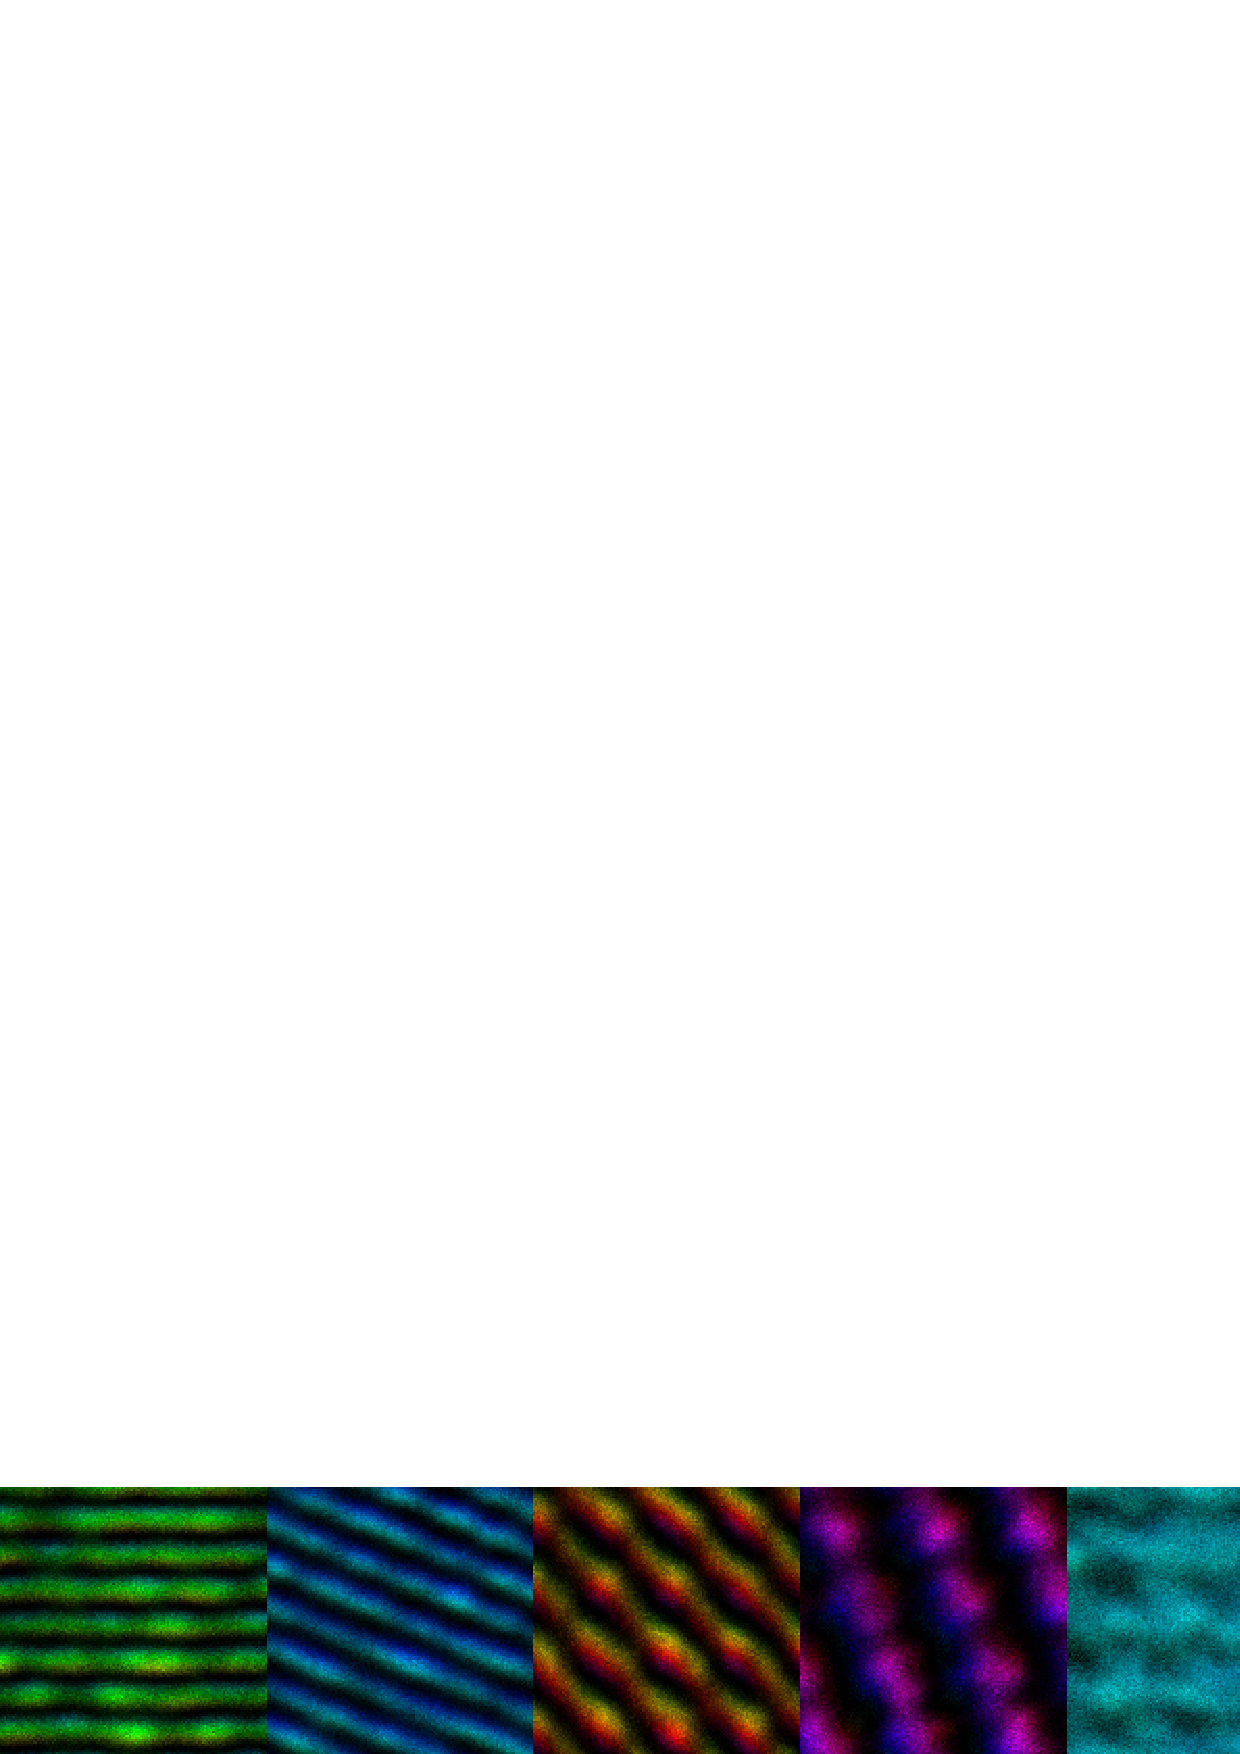
\includegraphics{tmp/out.pdf}
%\caption{How do the font sizes look?}
%\end{figure}


\part{The Centrifugal Force Quartz Crystal Microbalance}
\label{part:qcm}
\chapter{Foundations}
\section{Overview}
Mechanical properties such as viscoelasticity, contact stiffness and
adhesion, and force-dependent conforma- tional changes have been shown to
be instrumental in understanding biofunctional behavior from single
molecules to complex collections of cells. These properties are often
descriptive for specific molecules and cell types. For example, force
extension curves of DNA vary with assembly of histone proteins into
chromatin. In cells, viscoelasticity alone can discriminate between
healthy and cancerous tissue. Biosensors that can probe mechanical
properties are therefore ideal for both fundamental studies in life
sciences as well as diagnostic assays improving public health.

Perhaps the simplest way to probe a biomechanical property is by monitoring
its response to direct application of force. Current force based
approaches, for example those based on atomic force microscopy or optical
or magnetic tweezers, are powerful but limited in their applicability as
biosensors. In particular, their operation requires significant expertise
on the part of the investigator, and is often constrained to well prepared
samples not amenable to multiplexing.

Among tools suitable for direct mechanical transduction, the quartz crystal
microbalance (QCM) has seen increasing real-world utility as simple, cost
effective, and highly versatile mechanical biosensing platforms.  A QCM
typically manifests itself as a thin disk of piezoelectric quartz with
electrodes on either side.  The quartz is cut such that, when driven by a
potential, the crystal produces acoustic shear waves on either of its two
faces.  When a material is in contact with the crystal, its resonance
condition will change.  These changes can be used to interrogate both the
viscoelastic properties of the material and the way in which it is coupled
to the QCM.  This mechanical turns out to be extrorinary sensitive, even in
liquid environments, with sensitivities to mass on the order of X.  The
function of a QCM is depicted schematically in \Figure{fig:qcmschema}.

\begin{figure}
 \caption{Schematic representation of the operation of a QCM.  The
  quartz crystal is driven by a pair of electrodes on either sides to
  excite \si{\mega\hertz} acoustic shear waves.  A sample in contact with
  the crystal will typically change its resonant frequency $\df$ and
  bandwidth $\dg$, which are connected to the viscoelastic properites of
 the sample and the way in which it is coupled to the device.}
\end{figure}

Since its introduction by Sauerbrey [10] in 1959 as sub-monolayer thin-film
mass sensors in the gas phase, the understanding of these piezoelectric
devices has been repeatedly enhanced to study phenomena such as
viscoelastic films in the liquid phase [11], non-destructive contact
mechanics [12], and complex topolo- gies of biopolymers and
biomacromolecules [13]. However, despite their popularity QCMs suffer from
low-Q resonances which negatively impact their sensitivity. In addition,
extracting quantitative mechanical information from biomolecules is often
confounded by non-trivial interpretation of the discrete shifts in the
system's frequency and bandwidth.

The centrifugal force quartz crystal microbalance (CF-QCM), shown in
\Figure{fig:cfqcm} is our tool to do something.  The CF-QCM is a new type
of instrument which places a quartz crystal microbalance in a standard
commercial centrifuge.  When spinning, controllable centrifugal force is
applied to a biomaterial under assay, and the QCM signal as a function of
applied force is monitored in situ and in real time.

Where typical mechanical biosensing produces a single, stepwise sensor
response that can be linked to, in the case of a QCM, the static adsorbed
mass, contact stiffness, or viscoelastic compliance, our proposal allows
for the direct manipulation of elective dynamic versions of these
parameters through centrifugal force gradients.
Examples of loads which could be probed and the possible action of
centrifugal force are shown in \Figure{fig:cfqcm}
\begin{figure}
 \caption{Schematic of the CF-QCM.}
\end{figure}
\begin{table}
 \centering
\begin{tabular}{lll}
\toprule
& load & action\\
\midrule
(a)& monolayer of DNA molecules& change the conformal shape of DNA\\
(b)& protein coated microparticles& affect the contact stiffness\\
(c)& microparticles tethered with lambda DNA& extend and stretch DNA\\
(d)& heterogeneous collections of cells& modify cell adhesion and contact area\\
\bottomrule
\end{tabular}
\caption{Load situations depicted in \Figure{fig:cfqcm}}
\end{table}

\section{What is New Here}
QCMs have been studied in the context of almost every load situation
imaginable, but up to now the introduction and study of the behavior of
different load situations under uniform force gradients has not been
carried out.
The novel aspects of this work is the direct introduction of force
into\dots

\begin{description}
\item[{Acceleration Boundary Effects}] While the $kT$ energy of a
small biomolecule are orders of magnitude greater than gravity\todo{energy,
gravity, huh?}, acceleration effects are readily observable for hybridized
oligos and bufers stuff.  We confirm the 2g effect for oligos and provide
data into the 100g range, as well as confirm the effect for random buffer
solutions.
\item[{Contact Mechanics}] Pressing beads and looking at the response,
 maybe the equivalent model for contact stiffness in the liquid phase,
 which is just about shear stuffs.
\item[{one more thing so this list isn't empty}] That would be nice.
\end{description}

QCMs have been the subject of extensive study, especially in the context of
biosensing, and have for some time been implemented in commercial sensing
devices.  I will only cover areas related to new results here.  For a
comprehensive overview to the principles and applications of these
mechanical resonators, the reader is directed to \cite{steinemreview}.

\section{Historical Perspective}
As sensors, QCMs found their initial applications monitoring thin film
deposition in vacuums.  Here it was found that a QCM would exhibit a
frequency shift $\df$ proportional to the adsorbed mass $m$
\begin{equation}
 \df=-\frac{2f_{F}^{2}}{A\sqrt{\rho_{q}\mu_{q}}}\Delta m
 \label{eqn:sauerbrey}
\end{equation}
where $A$ is the active area of the crystal, $\Delta m$ is the adsorbed
mass, $\rho_{q}$ is the density of quartz and $\mu_{q}$ is the shear
modulus of quartz. Usually \Equation{eqn:sauerbrey} is condenced such that
$\Delta m$ is a linear function of a single ``sensitivity factor''
$C_\mathrm{f}$
\begin{equation}
 \Delta f=-C_{\text{f}}\Delta m
\end{equation}
where $C_{\text{f}}=\SI{56.6}{\hertz\per\micro\gram\centi\meter\squared}$.
\Equation{eqn:sauerbrey} is known as the
\textit{Sauerbrey relation}.  A typical QCM might have a
$f_F=\SI{5}{\mega\hertz}$ and a frequency resolution of \SI{0.1}{\hertz};
\Equation{eqn:sauerbrey} predicts sub-monolayer (and is only valid in this
range) resolution of the thickness
metal and dielectric layers.  This is the reason the name QCM includes the
word ``microbalance''.

Initially it was thought that the low $Q$ mechanical resonance of the QCM
precluded its use in the liquid phase.  This was incorrect, as subsequent
work published in 1985 by \name{Gordon} and \name{Kanazawa}~\cite{guys} extended the
treatment of \name{Sauerbrey} to the liquid phase.  These relations,
derived from a Butterworth van Dyke equivalent circuit, predicted the
resonant frequency of the QCM
to be sensitive to the density-viscosity product of the liquid in contact
with the crystal, 
\begin{align}
\df=&-f_{\text{F}}^{3/2}\left(\frac{\rho_{\text{L}}\eta_{\text{L}}}{\pi\rho_{q}\mu_{q}}\right)^{1/2}\\
\Delta R=&2f_{\text{F}}L\left(\frac{4\pi
 f_{\text{F}}\rho_{\text{L}}\eta_{\text{L}}}{\rho_{q}\mu_{q}}\right)^{1/2}
\end{align}
where $\rho_{\text{L}}$ and $\eta_{\text{L}}$ are the unknown density and
viscosity of the liquid.  Note that in the treatment by both Sauerbrey and
Gordon and Kanazawa, the frequency shifts are always \textit{negative} as a
function of increasing mass or density-viscosity.

The same year, \name{G. Dybwad} published a rather elegant
experiment~\cite{dybwad} in which he looked at the frequency shift of a QCM
in air when a single micron sized gold particle rests on the sensor
surface.  Remarkably, \name{Dybwad} reported a \textit{positive}
frequency shift.  The shift was explained with a coupled oscillator model
shown in \Figure{fig:dybwad}.
\begin{figure}
 \caption{Coupled oscillator model used by \name{Dybwad}.}
 \label{fig:dybwadschema}
\end{figure}
Here, the quartz crystal with mass $\mq$ and stiffness
$\kq$ resonates at
$\omega_\mathrm{q}^2=\kq/\mq$ and is coupled by a spring
$\kl$ to a load mass $\ml$.  The load mass is the actual mass of
the particle, $4/3 \pi r^3 \rho$.  The spring $\kl$ represents the
``stiffness'' of the contact -- how strongly the particle is coupled to the
QCM surface.  The coupled system in \Figure{fig:dybwadschema} is described
by the differential equations
\begin{align}
 \mq \ddot{x}_\mathrm{q} &= -\kq x_\mathrm{q}\\
 \ml \ddot{x}_\mathrm{L} &= -\kl (x_\mathrm{q}-x_\mathrm{L})
\end{align}
which, using an ansatz of
$x_{\mathrm{q},\mathrm{L}}=A_{\mathrm{q},\mathrm{L}}\me^{\mi \omega t}$ has
eigenvalues $\omega$ of
\begin{equation}
 2\omega^{2}=\left(\frac{\kq}{\mq}+\frac{\kl}{\mq}+\frac{\kl}{m}\right)\pm\left(\left(\frac{\kq}{\mq}+\frac{\kl}{\mq}+\frac{\kl}{\ml}\right)^{2}-4\frac{\kq}{\mq}\frac{\kl}{\ml}\right)^{1/2}
 \label{eqn:dybwadresult}
\end{equation}

\begin{figure}
 \caption{Resonant frequency of the Dybwad model as a function of coupling
  strength, $\kl$.}
 \label{fig:dybwadplot}
\end{figure}
\Equation{eqn:dybwadresult}, shown in \Figure{fig:dybwadplot} has two
important limits about $\omegaq^2 \ml$
\begin{align}
 \lim_{\kl\to\infty} \omega^2 &= \frac{\kq}{\mq+\ml}\\
 \lim_{\kl\to0} \omega^2 &= \frac{\kq}{\mq}
\end{align}
In the weak coupling regime, $\kl\ll\omegaq^2\ml$, the particle causes a
positive frequency shift proportional to $\kl$ and independent of $\ml$.
Indeeed, in \name{Dybwad}'s model, in the weak coupling regime the
particle is seen to be at rest in the labratory frame. In the limit of strong
coupling, $\kl\gg\omegaq^2\ml$, the mass adsorption predicted by
\name{Sauerbrey} takes over.  Dybwad's work is important because it
establishes a continuum model for QCM behavior, encompassing both positive
and negative frequency shifts.

Some dingus guys use a nanoindenter probe combined with a QCM, this is
where we jump off.

Last, Yuki got the idea from other applicaions of force on stuff done by
Ken and Wesley.  So plan to jump into the main text.

\section{DF Ratio}
\chapter{Experimental Setup}
The experimental setup consists of a 
\section{Mechanical}
\subsection{Centrifuge}
\subsection{Microfluidic Cell}
\subsection{Mounting and Stress}

\section{Driving Circuit}
The QCM driving circuit employed in our experiments was an SRS 

\section{Chemistry and Surface Functionalization}
\subsection{Cleaning the Crystals}

\chapter{Load Situations}
\section{Environmental Effects and Sources of Noise}
\subsection{Temperature Drift}
\section{Air}
\section{Deionized Water}
\section{Salt Buffers}
\section{Microparticles}
magnetic lift off
different radii
\section{Lambda DNA}
\section{Oligo Attached Particles}
\section{Particles Tethered to the Surface with Lambda DNA}

\chapter{Strange Effects}
\section{Bubble Resonance}

\chapter{Future Work}

\part{Appendix}
\appendix

\chapter{Miscellaneous}
\section{Colophon}
This document was typeset using pdf\TeX. All
plots were rendered using pgfplots~\cite{feuersangerpgfplots} with styles influenced by
\name{Eduard~Tufte}~\cite{tufte1983visual}~\cite{tufte1991envisioning}. Colors were chosen
from datasets researched by \name{Jan~Brewer}~\cite{harrower2003colorbrewer}.
Schematics and other line drawings were prepared using Inkscape. Generation
of text was done under Arch Linux using \texttt{vim}.  Some tables were
pre-processed using LyX.

The Monte Carlo simulations were written in \texttt{c} with parallelism
accomplished using \texttt{mpi}. The vortex tracking and image processing
algorithms were written in \texttt{octave}.  Weirdospace images were
processed using python and scipy/numpy.  Parallel execution when required
was done at at the FAU RRZE, Erlangen, Germany.  Multiple scattering code
written by \name{Matthew~Foreman} was written in \texttt{MATLAB}.  All sources
available through the author.

\chapter{Protocols}
\section{Sputtering}
\section{Functionalizing Nanoparticles}
\section{Microfluidics}
\section{Sping Coating of Cytop}

\chapter{Reference Data}
Several datasets were produced during the course of this dissertation which
might be useful to the reader.  They are presented here.
\section{Physical Properties of SPP Propagation}
\label{ref:physicalproperties}
%\import{dispersion/}{sptable_632.tex}
\section{The Three Layer Fresnel System}
%% you will have to fix the path in the following file
%\import{fresnel_plots/}{allthreelayerfresnel}

\section{Complex Permittivities and Permiabilities of Metals}
%\import{eps_plots/}{allmetals}


\section{Abbreviations}
%\begin{table}
% \begin{tabular}
%  SPP & surface plasmon polariton
%  LRSPP & long range surface plasmon polariton
% \end{tabular}
%\end{table}

\bibliographystyle{plain}
\bibliography{bibliography}

\listoftodos
\end{document}

% MISSING A HOME
% surface roughness parameters
